% Poster figure (left column): DfpNet as a U with the block insertion points (top) and the residual SS2D block
% (bottom). Standalone TikZ, Helvetica + sansmath, drawn at its poster size (16.2 x 6.3 cm, text 12 pt): include with
% 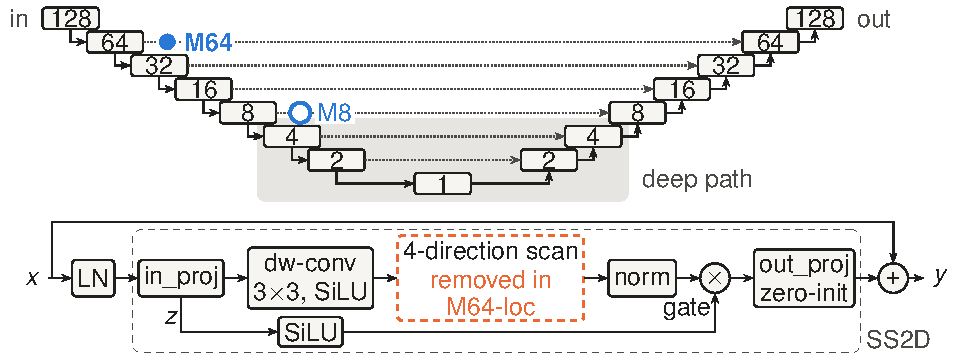
\includegraphics[width=\linewidth]{fig_block.pdf} in the 16.2 cm column (no scaling).
% Caption should say: boxes = feature-map size s (s x s), in = mask and free-stream velocity, out = p, v_x, v_y;
% in M64-loc the scan is replaced by its skip term D * u.
% Facts from CLAUDE.md and docs/lab-notebook.md (night 6b: deep path = layer4-6 / dlayer6-4, below 8x8; nights 8 / 9:
% MDv block after layer1 at 64x64, MDv64-local without the scan, out_proj zero-initialised).
\documentclass[border=0.5pt]{standalone}
\usepackage[T1]{fontenc}
\usepackage{helvet}
\renewcommand{\familydefault}{\sfdefault}
\usepackage{sansmath}
\usepackage{tikz}
\usetikzlibrary{arrows.meta, positioning, fit, backgrounds, calc}

% palette shared with scripts/poster_figures.py
\definecolor{mblue}{HTML}{2A78D6}
\definecolor{morange}{HTML}{EB6834}
\definecolor{ink}{HTML}{1F1F1E}
\definecolor{muted}{HTML}{4A4A47}
\definecolor{deep}{HTML}{E6E5E1}
\definecolor{boxfill}{HTML}{F6F5F2}

\begin{document}
\fontsize{12}{14}\selectfont\sansmath
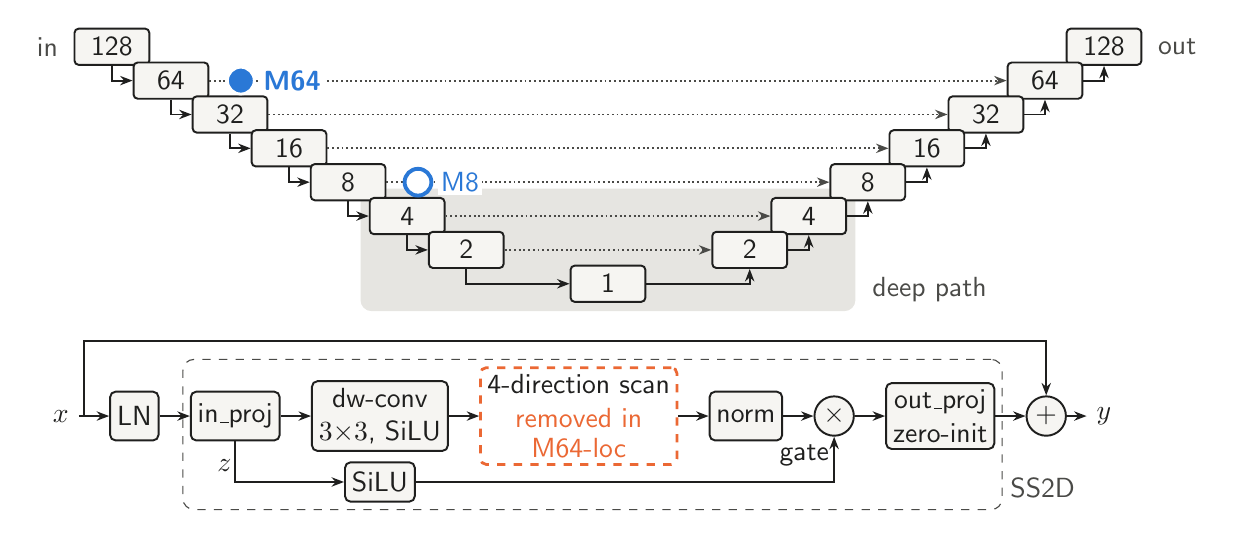
\begin{tikzpicture}[
    >={Stealth[length=4.5pt]}, line width=0.7pt, draw=ink, text=ink,
    lvl/.style={draw=ink, fill=boxfill, rounded corners=1.5pt, minimum height=0.46cm, minimum width=0.95cm,
                inner sep=1pt},
    op/.style={draw=ink, fill=boxfill, rounded corners=2pt, minimum height=0.62cm, inner sep=2.5pt, align=center},
    ins/.style={circle, fill=mblue, draw=white, line width=1pt, minimum size=0.34cm, inner sep=0pt},
    skip/.style={densely dotted, muted, line width=0.7pt, ->},
  ]

  % ---------------- U-Net (DfpNet, expo 5): encoder left, decoder right; boxes = map size ----------------
  \def\dx{0.75}
  \def\dy{-0.43}
  \def\xd{12.6}
  \foreach \i/\s in {0/128, 1/64, 2/32, 3/16, 4/8, 5/4, 6/2} {
    \node[lvl] (e\i) at ({\dx*\i}, {\dy*\i}) {\s};
    \node[lvl] (d\i) at ({\xd-\dx*\i}, {\dy*\i}) {\s};
  }
  \node[lvl] (bn) at ({\xd/2}, {\dy*7}) {1};
  \foreach \i [evaluate=\i as \j using int(\i+1)] in {0,...,5} {
    \draw[->] (e\i.south) |- (e\j.west);
    \draw[->] (d\j.east) -| (d\i.south);
  }
  \draw[->] (e6.south) |- (bn.west);
  \draw[->] (bn.east) -| (d6.south);
  \foreach \i in {1,...,6} { \draw[skip] (e\i.east) -- (d\i.west); }
  \node[muted, left=2pt of e0] {in};
  \node[muted, right=2pt of d0] {out};

  % deep path (layer4-6, dlayer6-4: below 8x8) shaded
  \begin{scope}[on background layer]
    \node[fill=deep, rounded corners=4pt, inner sep=3pt, fit=(e5)(d5)(bn)] (deeppath) {};
  \end{scope}
  \node[muted, anchor=south west] at ($(deeppath.south east)+(0.08,0)$) {deep path};

  % insertion points: after layer1 (64x64, encoder) and at 8x8
  \node[ins] (i64) at ($(e1.east)+(0.4,0)$) {};
  \node[ins, fill=white, draw=mblue, line width=1.4pt] (i8) at ($(e4.east)+(0.4,0)$) {};
  \node[mblue, anchor=west, font=\bfseries, fill=white, inner sep=1pt] at ($(i64.east)+(0.05,0)$) {M64};
  \node[mblue, anchor=west, fill=white, inner sep=1pt] at ($(i8.east)+(0.05,0)$) {M8};

  % ---------------- residual block x + Mixer(LN(x)) with SS2D ----------------
  \begin{scope}[yshift=-4.69cm]
    \node (x) at (-0.65, 0) {$x$};
    \node[op, right=0.385cm of x] (ln) {LN};
    \node[op, right=0.385cm of ln] (inp) {in\_proj};
    \node[op, right=0.385cm of inp] (dw) {dw-conv\\ $3{\times}3$, SiLU};
    \node[op, right=0.385cm of dw, draw=morange, dashed, line width=1pt, fill=white] (scan)
      {4-direction scan\\ \textcolor{morange}{removed in}\\[-1pt] \textcolor{morange}{M64-loc}};
    \node[op, right=0.385cm of scan] (norm) {norm};
    \node[op, right=0.385cm of norm, circle, minimum height=0.5cm, inner sep=0pt] (mul) {$\times$};
    \node[op, right=0.385cm of mul] (outp) {out\_proj\\ zero-init};
    \node[op, right=0.385cm of outp, circle, minimum height=0.5cm, inner sep=0pt] (add) {$+$};
    \node[right=0.25cm of add] (y) {$y$};

    \draw[->] (x) -- (ln);
    \draw[->] (ln) -- (inp);
    \draw[->] (inp) -- (dw);
    \draw[->] (dw) -- (scan);
    \draw[->] (scan) -- (norm);
    \draw[->] (norm) -- (mul);
    \draw[->] (mul) -- (outp);
    \draw[->] (outp) -- (add);
    \draw[->] (add) -- (y);
    % gating branch z -> SiLU -> x
    \node[op, below=0.12cm of dw, minimum height=0.5cm] (silu) {SiLU};
    \draw[->] (inp.south) |- node[pos=0.3, left, inner sep=1pt] {$z$} (silu.west);
    \draw[->] (silu.east) -| node[pos=0.8, left, inner sep=1.5pt] {gate} (mul.south);
    % residual path
    \draw[->] ($(x.east)+(0.06,0)$) -- ++(0,0.95) -| (add.north);

    \begin{scope}[on background layer]
      \node[draw=muted, dashed, rounded corners=4pt, inner sep=2.5pt, fit=(inp)(outp)(silu)(scan)] (mixer) {};
    \end{scope}
    \node[muted, anchor=north west, inner sep=1pt] at ($(mixer.south east)+(0.05,0.45)$) {SS2D};
  \end{scope}
\end{tikzpicture}
\end{document}
